 
 
\subsection{Función solver set bnd}
 
Se evaluó el código en assembler, llamado asm, y código c de la función solver set bound sobre seis tamaños distintos de matrices. al variar parámetro b, valores de 1,2,3 y 10, se obtienen promedios similares en caso de matriz con tamaño 512x512 (ver tabla), sacando outliers. Los resultados se mantienen alrededor de 18500 ticks para asm y 54000 ticks para c. 
Repetimos escenario con matriz de tamaño 16x16, variando b en mismos valores que para tamaño 512x512. Aunque se nota 
variación de tiempos entre mediciones no se nota gran cambio en los resultados, manteniendose el promedio de tiempos c alrededor de 2000 ticks y tiempos asm alrededor de 350 ticks.
\begin{table}[htbp]
\begin{center}
\begin{tabular}{|l|l|l|}
\hline
  & C & ASM\\
\hline \hline
$solver\_set\_bnd\_100\_16\_b1$ & 2061.989474 & 335.134021\\ \hline
$solver\_set\_bnd\_100\_16\_b2$  & 2081.364583 & 360.896907\\ \hline
$solver\_set\_bnd\_100\_16\_b3$  & 2068.020408 & 376.135417 \\ 
\hline \hline
$solver\_set\_bnd\_100\_512\_b1$  & 56134.061856 & 18529.938144 \\ \hline

$solver\_set\_bnd\_100\_512\_b2$  & 54054.041667 & 19752.25000 \\ \hline

$solver\_set\_bnd\_100\_512\_b3$  &  54835.708333 & 18544.926316 \\ \hline

\end{tabular}
\caption{Tabla de promedios ticks función solver set bnd para tamaños 16x16 y 512x512.}
%\label{tabla:sencilla}
\end{center}
\end{table}
A causa de esto y de que no queremos llenar de gráficas innecesarias hemos decidido fijar el parámetro b en 2 para restantes experimentaciones de función. 
se muestra en figura gráfica de ejecución de los códigos, donde para cada tamaño se ejecutaron 100 veces.
\begin{figure}[h]

\centering
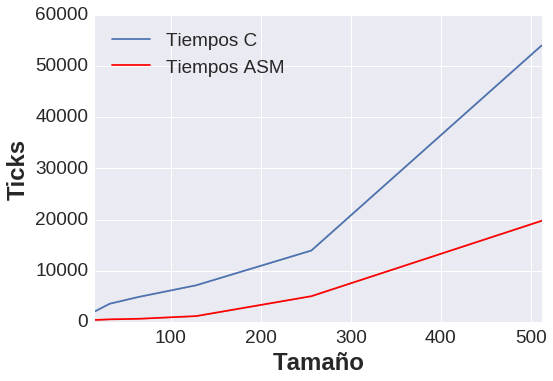
\includegraphics[scale=0.6] {grafica_set_bound}
  
 \caption{Tiempos en ticks de ejecución de código C vs código ASM para función solver set bnd}
\end{figure} 

\subsection{Función solver lin solve}
hemos variado los parámetros a,b y c para tamaños de matriz 16 y 512. En la tabla siguiente se muestran los promedios obtenidos sobre datos sin outliers para valores de: a = 1.0f y c = 4.0f, llamado 1erOp-a-y-c, a = 0.3f y c = 2.8f, llamado 2daOp-a-y-c, y a = -10.0f, c = 0.02f, llamado 3raOp-a-y-c. Los valores de b son: 1, 2, 3 y 10. En el caso de tamaño 16 obtenemos que el promedio de tiempos de ejecución sin outliers para código en C está alrededor de los 400000 ticks y para código asm está alrededor de 300000 ticks. En el caso de tamaño 512 se obtiene que promedio de tiempos C está alrededor de 2.3*e+08 y tiempos asm está alrededor de 1.6*e+08 ticks.
\begin{table}[htbp]
\begin{center}
\begin{tabular}{|l|l|l|}
\hline
  & C & ASM\\
\hline \hline
$solver\_lin\_solve\_b1\_1erOp\_a\_y\_c\_16$ & 392938.224490 & 236550.530612\\ \hline

$solver\_lin\_solve\_b2\_1erOp\_a\_y\_c\_16$ & 442471.040816 & 252094.406250\\ \hline

$solver\_lin\_solve\_b3\_1erOp\_a\_y\_c\_16$ & 429083.391753 & 253708.344086\\ \hline

$solver\_lin\_solve\_b10\_1erOp\_a\_y\_c\_16$ & 436142.561224  & 261522.363636\\ \hline


$solver\_lin\_solve\_b1\_2daOp\_a\_y\_c\_16$ & 461250.443299 & 369954.084211\\ \hline

$solver\_lin\_solve\_b10\_2daOp\_a\_y\_c\_16$ & 430715.626263 & 352677.979592\\ \hline

$solver\_lin\_solve\_b1\_3raOp\_a\_y\_c\_16$ & 427202.773196  & 262558.585859\\ \hline


$solver\_lin\_solve\_b10\_3raOp\_a\_y\_c\_16$ & 429630.377551    & 237256.265306\\ \hline

\hline \hline 


$solver\_lin\_solve\_b1\_1raOp\_a\_y\_c\_512$ & 2.320231e+08  & 1.576663e+08\\ \hline

$solver\_lin\_solve\_b2\_1raOp\_a\_y\_c\_512$ & 2.364991e+08  &  1.582853e+08\\ \hline

$solver\_lin\_solve\_b10\_1raOp\_a\_y\_c\_512$ & 2.313464e+08   &  1.570360e+08\\ \hline

$solver\_lin\_solve\_b1\_3raOp\_a\_y\_c\_512$ & 2.343117e+08  & 1.585373e+08\\ \hline

$solver\_lin\_solve\_b10\_3raOp\_a\_y\_c\_512$ & 2.337076e+08 & 1.611139e+08\\ \hline

\end{tabular}
\caption{Tabla de promedios ticks función solver lin solve para tamaños 16x16 y 512x512.}
%\label{tabla:sencilla}
\end{center}
\end{table}
 Se ve en la tabla que se repite una proporción de casi el doble gasto temporal en ejecuciones C respecto a ejecuciones asm. Entonces decidimos elegir parámetros de 1erOp-a-y-c, b = 2 y las matrices solver-u, solver-v. Con estos parámetros variamos el tamaño de las matrices y graficamos los tiempos (ver gráfica).
\begin{figure}[h]

\centering
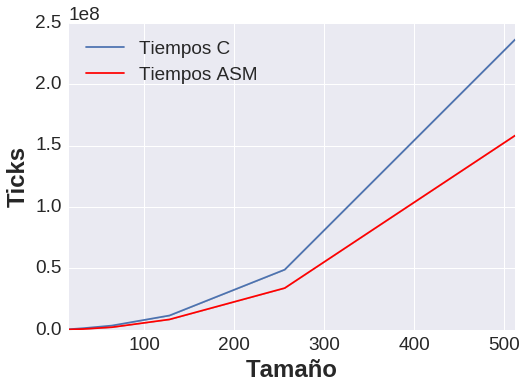
\includegraphics[scale=0.6] {solver_lin_solve}
  
 \caption{Tiempos en ticks de ejecución de código C vs código ASM para función solver lin solve}
\end{figure} 

\subsection{Función solver project}
Hemos medido la función sobre cuatro matrices diferentes: 1erOp que comienza con valor (0.1,0.2) en posición (0,0) y luego a medida que avanza en posiciones se incrementa en uno y se les asigna el resultado, 2daOp con mismo proceso pero comenzando en (0.09,-100), 3eraOp comenzando en (-10,0.08) y 4taOp comenzando en (1000,2000). Se evalúan matrices con tamaño 16 y 512 para observar si hay gran cambio en las proporciones de tiempo al ejecutar código. Se observa en tabla los resultados y se ve que 
para ambos tamaños el código C gasta alrededor de un tercio más que tiempo gastado por código asm. 
 

\begin{table}[htbp]
\begin{center}
\begin{tabular}{|l|l|l|l|l|}
\hline
  & C &  SD(c) & ASM & SD(asm)\\
\hline \hline

$solver\_project\_1erOp\_matrices\_16$ & 384948.313131 & 36503.785424 & 271883.232323 & 28601.904704\\ \hline
 
$solver\_project\_2daOp\_matrices\_16$ & 385072.787879 & 34959.635332 & 271078.418367 & 15269.103250\\ \hline

$solver\_project\_3eraOp\_matrices\_16$ & 382180.464646 & 29999.207094  & 273869.231579 & 13431.150139\\ \hline

$solver\_project\_4taOp\_matrices\_16$ & 353107.683673 & 24055.789775    & 259020.680412 & 12374.032677\\ \hline
\hline \hline
 
$solver\_project\_1erOp\_matrices\_512$ & 1.925452e+08 &  1.804747e+06   & 1.584625e+08 & 1.589767e+06\\ \hline

$solver\_project\_2daOp\_matrices\_512$ & 1.939796e+08 &  3.205834e+06   & 1.591681e+08 & 2.147394e+06\\ \hline


$solver\_project\_4taOp\_matrices\_512$ & 1.938470e+08 & 2.764452e+06   & 1.670031e+08 & 8.623912e+06\\ \hline

\end{tabular}
\caption{Tabla de promedios ticks función solver project para tamaños 16x16 y 512x512.}
%\label{tabla:sencilla}
\end{center}
\end{table}
A causa de que al variar la matriz obtenemos resultados similares, alrededor de 380000 ticks en código C y alrededor de 270000 en asm para tamaño 16 (ver tabla), hemos decidido evaluar los códigos sobre matriz 1erOp. En la gráfica se muestran los promedios para distintos tamaños.
\begin{figure}[h]

\centering
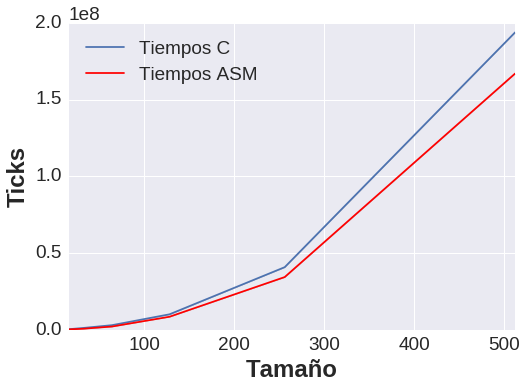
\includegraphics[scale=0.6] {solver_project}
   \caption{Tiempos en ticks de ejecución de código C vs código ASM para función solver project}
\end{figure}




